\documentclass[cvauthor={Dr. Sajid Muhaimin Choudhury}]{buetcv}

\bibliography{papers} 
\begin{document}
    \placelastupdatedtext %last when updated
    \begin{header}
        \fontsize{30 pt}{30 pt}
        \textbf{\cvauthor}

        \vspace{0.2 cm}
        \fontsize{20 pt}{20 pt}
        Associate Professor, Department of EEE, BUET \\
        \vspace{0.2 cm}        
        \normalsize
        \mbox{{\footnotesize\faMapMarker*}\hspace*{0.13cm}Dhaka, Bangladesh}%
        \kern 0.25 cm%
        \AND%
        \kern 0.25 cm%
        \mbox{\hrefWithoutArrow{mailto:sajid@eee.buet.ac.bd}{{\footnotesize\faEnvelope[regular]}\hspace*{0.13cm}sajid@eee.buet.ac.bd}}%
        \kern 0.25 cm%
        \AND%
%        \kern 0.25 cm%
%        \mbox{\hrefWithoutArrow{tel:+90-541-999-99-99}{{\footnotesize\faPhone*}\hspace*{0.13cm}0541 999 99 99}}%
%        \kern 0.25 cm%
%        \AND%
        \kern 0.25 cm%
        \mbox{\hrefWithoutArrow{https://sajid.buet.ac.bd}{{\footnotesize\faLink}\hspace*{0.13cm}sajid.buet.ac.bd}}%
        \kern 0.25 cm%
        \AND%
        \kern 0.25 cm%
        \mbox{\hrefWithoutArrow{https://linkedin.com/in/sajidmc}{{\footnotesize\faLinkedinIn}\hspace*{0.13cm}sajidmc}}%
        \kern 0.25 cm%
    \end{header}

    \vspace{0.3 cm - 0.3 cm}


    \section{Brief Biography}
        \begin{onecolentry}
            Dr. Sajid Choudhury is working as an Associate Professor in the Department of EEE, BUET. Dr. Choudhury completed his Ph.D. from the School of Electrical and Computer Engineering in Purdue University. Dr. Choudhury had the privilege of acquiring skills of both experimental and numerical approaches to solve problems related to photonics. His current research interest is in Photonic Quantum Computing, Flat Optics with Metasurface, Photonic Devices with Phase Change Materials, Embedded Systems Design. He seeks to solve fundamental and high-impact research questions of photonics and quantum computing, as well as to design practical solutions to meet the needs of Bangladesh. Dr. Choudhury is a member of the Department of EEE, BUET Self Assessment Committee, seeking to improve and excel the educational quality of the department. He actively engages and volunteers in Professional societies. Dr. Choudhury is the Educational Activities Chair of IEEE Bangladesh Section, Chair, IEEE Photonics Society Bangladesh Chapter and founding President, The Optica Bangladesh Section. Dr. Choudhury is a senior member of the IEEE and member of Optica. He is a member of the National Young Academy of Bangladesh (NYAB).
        \end{onecolentry}



\section{Education}
        \begin{threecolentry}{\textbf{Ph.D.}}{
            Aug 2013 – Aug 2019
        }
            \textbf{Purdue University}, West Lafayette, IN, USA \\ School of Electrical and Computer Engineering
            \begin{highlights}
                \item \textbf{Ph.D. Thesis:} WAVEFRONT MANIPULATION WITH METASURFACES BASED ON NEW MATERIALS                 
                \item \textbf{Ph.D. Co-supervisor(s):} Alexandra Boltasseva and \\ Alexander Kildishev
            \end{highlights}
        \end{threecolentry}
        \begin{threecolentry}{\textbf{M.Sc. }}{
            Aug 2011 – 2013
        }
        \textbf{Bangladesh University of Engineeing and Technology (BUET)} \\ Department of Electrical and Electronic Engineering
            \begin{highlights}
                \item \textbf{M.Sc. Engg. Thesis:} Design of a Fractal Antenna based on Hexaflake Fractal Structure                 
                \item \textbf{M.Sc. Engg. Supervisor:} Dr. M. A. Matin 
            \end{highlights}
        \end{threecolentry}
        \begin{threecolentry}{\textbf{B.Sc.}}{
            Dec 2004 – Aug 2010
        }
            \textbf{Bangladesh University of Engineeing and Technology (BUET)} \\ Department of Electrical and Electronic Engineering
            \begin{highlights}
                \item CGPA: 3.94/4.0 
                \item \textbf{Undergraduate Thesis:} Design and Analysis of a Multiband Dual Feed Axially Symmetric Cassegrain Antenna System
                \item \textbf{Undergraduate Supervisor:} Dr. M. A. Matin 
            \end{highlights}
        \end{threecolentry}

        \begin{threecolentry}{\textbf{H.S.C.}}{
            2004
        }
            \textbf{Notre Dame College}, Dhaka 
            \begin{highlights}
                \item GPA: 5.00/5.00 
            \end{highlights}
        \end{threecolentry}
        \begin{threecolentry}{\textbf{S.S.C.}}{
            2002
        }
            \textbf{Udayan Uchchya Madhyamic Bidyalaya}, Dhaka 
            \begin{highlights}
                \item GPA: 5.00/5.00 
            \end{highlights}
        \end{threecolentry}        


    
\section{Experience}
        \begin{twocolentry}{
        July 2022 – to date 
        }
        Associate Professor, Department of Electrical and Electronic Engineering (EEE) \\ \textbf{Bangladesh University of Engineering and Technology (BUET)} \\
            %\begin{highlights}
            %    \item Reduced time to render user buddy lists by 75\% by implementing a prediction algorithm
            %    \item Integrated iChat with Spotlight Search by creating a tool to extract metadata from saved chat transcripts and provide metadata to a system-wide search database
            %\end{highlights}
        \end{twocolentry}
        \vspace{0.2 cm}
        \begin{twocolentry}{
            June 2013 – July 2022
            }
            Assistant Professor, Department of Electrical and Electronic Engineering (EEE) \\ \textbf{Bangladesh University of Engineering and Technology (BUET)} \\
        \end{twocolentry}

        \begin{twocolentry}{
            Jan 2010 – June 2013
            }
            Lecturer, Department of Electrical and Electronic Engineering (EEE) \\ \textbf{Bangladesh University of Engineering and Technology (BUET)}\\
        \end{twocolentry}

        \begin{twocolentry}{
            Nov 2011 – Jan 2010
            }
            Lecturer, Institute of Information and Communication Technology (IICT) \\ \textbf{Bangladesh University of Engineering and Technology (BUET)}\\
        \end{twocolentry}        
    
        
\section{Publications}
\vspace{0.2 cm}
\subsection{Publications Metrics}
% gscholar.tex
% ─────────────────────────────────────────────────────────────────
% This file defines a single floating figure containing:
%  - (a) a table of Google Scholar metrics
%  - (b) a bar chart of citations per year
%
% It assumes booktabs, pgfplots & subcaption are already loaded.
% ─────────────────────────────────────────────────────────────────

% gscholar.tex
%\documentclass[cvauthor={Dr. Sajid Muhaimin Choudhury}]{buetcv}
%\begin{document}
\begin{figure}[ht]
    \centering
    % ───── Panel (a): Table ─────
    \begin{subfigure}[t]{0.48\textwidth}
      \centering
      \caption{\aiGoogleScholar Google Scholar Metrics}
      \begin{tabular}{lrr}
        
           &   \\
        \midrule
        Total Citations & 1113  \\
        h-index & 12   \\
        i10-index & 10   \\
        \bottomrule
      \end{tabular}
    \end{subfigure}\hfill
    % ───── Panel (b): Bar chart ─────
    \begin{subfigure}[t]{0.48\textwidth}
      \small
      \centering
      \caption{\aiGoogleScholar Google Scholar Citations per Year}
      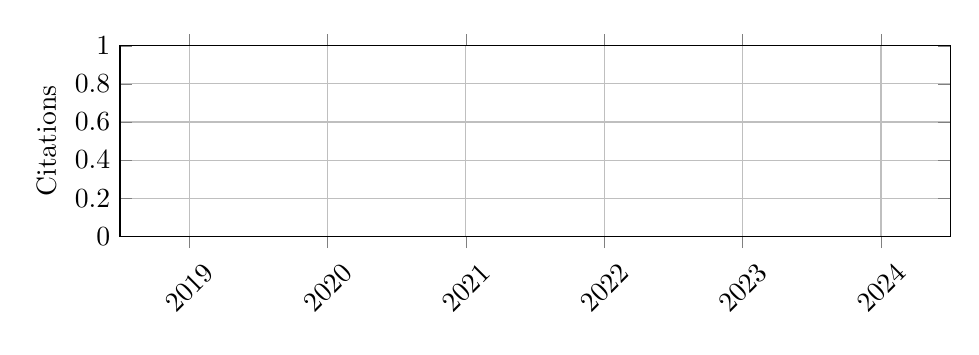
\begin{tikzpicture}
        \begin{axis}[
            width=\linewidth,% make the plot fill the subfigure width...
            height=4cm, % …but only 6 cm tall
            ybar,
            bar width=10pt,
            enlarge x limits=0.1,
            ylabel={\aiGoogleScholar Citations},
            ymin=0, ymax=220,
            ytick={ 0,55,110,165,220 },
            xtick=data,
            xticklabels={ 2018,2019,2020,2021,2022,2023,2024,2025 },
            % rotate the x‐tick labels:
            xticklabel style={rotate=45,anchor=near xticklabel},
            grid=major
          ]
          \                                                                  addplot[fill=gray] coordinates { (2018,41) (2019,67) (2020,151) (2021,171) (2022,207) (2023,168) (2024,184) (2025,57) };
        \end{axis}
      \end{tikzpicture}
    \end{subfigure}
  \end{figure}
%  \end{document}
\vspace{0.2 cm}   
    %\nocite{*}
    %\printbibliography
    %\printbibheading
\subsection{Journal Articles}
\csnumgdef{entrycount}{0}
\nocite{*}
\newrefcontext[labelprefix=J]
\printbibliography[env=counter,type=article,heading=none]

  \printbibliography[type=article,heading=none]



\subsection{Conference Proceedings}
\csnumgdef{entrycount}{0}
\nocite{*}
\newrefcontext[labelprefix=C]
\printbibliography[env=counter,type=inproceedings,heading=none]
\printbibliography[type=inproceedings,heading=none]


\subsection{Patents}
\csnumgdef{entrycount}{0}
\nocite{*}
\newrefcontext[labelprefix=P]
\printbibliography[env=counter,type=patent,heading=none]
\printbibliography[type=patent,heading=none]

\subsection{Preprint / Manuscript Under Preparation}
\csnumgdef{entrycount}{0}
\nocite{*}
\newrefcontext[labelprefix=X]
\printbibliography[env=counter,type=unpublished,heading=none]
\printbibliography[type=unpublished,heading=none]


\section{Membership / Fellowship of Learned Societies, Professional Institutions and Other Noteworthy Affiliations}
        \begin{onecolentry}
            \textbf{Senior Member, Institute of Electrical and Electronic Engineers (IEEE)}
            \begin{highlights}
                \item Secretary, IEEE Bangladesh Section (July 2021 - May 2022)
                \item Chair, IEEE Young Professionals Bangladesh	(Mar 2020 - Apr 2022)
                \item Chair, IEEE Graduates of the Last Decade	(Jan 2013 - Dec 2013)
                \item Vice -Chair, IEEE Graduates of the Last Decade	(Jan 2011 - Dec 2012)
                \item Student Activities Coordinator, IEEE Bangladesh Section	(Jan 2011 - Dec 2012)
                \item Chair, IEEE BUET Student Branch	(Jan 2008 - Aug 2009)
                \item Treasurer, IEEE BUET Student Branch	(Jan 2007 - Dec 2008)
            \end{highlights}
        \end{onecolentry}
        \begin{onecolentry}
            \textbf{Member, IEEE Photonics Society}
            \begin{highlights}
                \item Vice Chair, IEEE Photonics Society Bangladesh	(April 2022 – to date)
                \item Founding Chair, IEEE Photonics Society Bangladesh	(Mar 2021 – Apr 2022)
                \end{highlights}
            \end{onecolentry}
            \begin{onecolentry}
                \textbf{Member, The Optica}
                \begin{highlights}
                \item Founding President, Optica Bangladesh Section	May 2022 – to date
                \item Founding Moderator, BUET Optical and Photonics Society 	July 2022 – to date 
                \item Treasurer, OSA Purdue Chapter, USA	Jun 2016 – May 2017
            \end{highlights}
            \end{onecolentry}        
            \begin{onecolentry}
                \textbf{Member, National Young Academy of Bangladesh (NYAB)}, April 2021 – to date    \\     
                \textbf{Life Member, American Alumni Association of Bangladesh (AAAB)	}, April 2024 – to date    
                \\                    
                \textbf{Life Member, Association of BUET Alumni}, April 2021 – to date    \\     

        \end{onecolentry} 
        \begin{onecolentry}
            \textbf{Student Activities at Purdue University}, West Lafayette, IN, USA
            \begin{highlights}
                \item President, \textbf{Nanotechnology Student Advisory Council (NSAC)}	(Jun 2017 – May 2018)
                \item Vice-President, \textbf{Nanotechnology Student Advisory Council (NSAC)}	(Jun 2016 – May 2017)
                \item Treasurer, SPIE Purdue Chapter, USA (Jun 2015 – May 2016)
                \item President, Bangladesh Students Association (\textbf{Purdue BDSA}), USA  (Jul 2017 – Jun 2018)
                \item Treasurer, Bangladesh Students Association (\textbf{Purdue BDSA}), USA  (Jul 2015 – Jun 2017)
            \end{highlights}
        \end{onecolentry} 

        \vspace{0.2 cm}
    
\section{References}

Available upon request

    

\end{document}